%% Creator: Inkscape 1.3.2 (091e20e, 2023-11-25), www.inkscape.org
%% PDF/EPS/PS + LaTeX output extension by Johan Engelen, 2010
%% Accompanies image file 'figures/ch5/hbm-math-diagram.pdf' (pdf, eps, ps)
%%
%% To include the image in your LaTeX document, write
%%   \input{<filename>.pdf_tex}
%%  instead of
%%   \includegraphics{<filename>.pdf}
%% To scale the image, write
%%   \def\svgwidth{<desired width>}
%%   \input{<filename>.pdf_tex}
%%  instead of
%%   \includegraphics[width=<desired width>]{<filename>.pdf}
%%
%% Images with a different path to the parent latex file can
%% be accessed with the `import' package (which may need to be
%% installed) using
%%   \usepackage{import}
%% in the preamble, and then including the image with
%%   \import{<path to file>}{<filename>.pdf_tex}
%% Alternatively, one can specify
%%   \graphicspath{{<path to file>/}}
%% 
%% For more information, please see info/svg-inkscape on CTAN:
%%   http://tug.ctan.org/tex-archive/info/svg-inkscape
%%
\begingroup%
  \makeatletter%
  \providecommand\color[2][]{%
    \errmessage{(Inkscape) Color is used for the text in Inkscape, but the package 'color.sty' is not loaded}%
    \renewcommand\color[2][]{}%
  }%
  \providecommand\transparent[1]{%
    \errmessage{(Inkscape) Transparency is used (non-zero) for the text in Inkscape, but the package 'transparent.sty' is not loaded}%
    \renewcommand\transparent[1]{}%
  }%
  \providecommand\rotatebox[2]{#2}%
  \newcommand*\fsize{8 pt\relax}%
  \newcommand*\lineheight[1]{\fontsize{\fsize}{#1\fsize}\selectfont}%
  \ifx\svgwidth\undefined%
    \setlength{\unitlength}{263.77443695bp}%
    \ifx\svgscale\undefined%
      \relax%
    \else%
      \setlength{\unitlength}{\unitlength * \real{\svgscale}}%
    \fi%
  \else%
    \setlength{\unitlength}{\svgwidth}%
  \fi%
  \global\let\svgwidth\undefined%
  \global\let\svgscale\undefined%
  \makeatother%
  \begin{picture}(1,0.56827175)%
    \lineheight{1}%
    \setlength\tabcolsep{0pt}%
    \put(0,0){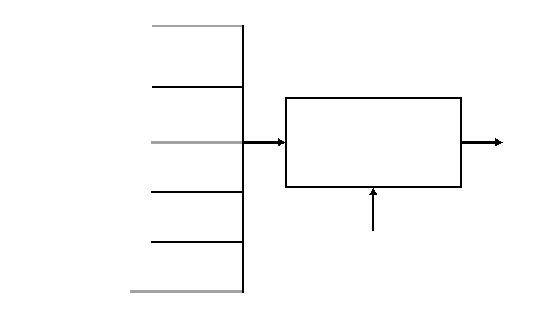
\includegraphics[width=\unitlength,page=1]{figures/ch5/hbm-math-diagram.pdf}}%
    \put(-0.00172156,0.5140235){\color{black}\makebox(0,0)[lt]{\lineheight{1.25}\smash{\begin{tabular}[t]{l}$i=1$\end{tabular}}}}%
    \put(-0.00172156,0.40289279){\color[rgb]{0,0,0}\makebox(0,0)[lt]{\lineheight{1.25}\smash{\begin{tabular}[t]{l}$i=2$\end{tabular}}}}%
    \put(-0.00172156,0.30206003){\color[rgb]{0,0,0}\makebox(0,0)[lt]{\lineheight{1.25}\smash{\begin{tabular}[t]{l}$i=3$\end{tabular}}}}%
    \put(0.5337258,0.30917476){\color[rgb]{0,0,0}\makebox(0,0)[lt]{\lineheight{1.25}\smash{\begin{tabular}[t]{l}$\frac{\text{OR}_0\cdot\text{OR}_2\cdot\text{OR}_4\cdot\text{OR}_5}{1+\text{OR}_0\cdot\text{OR}_2\cdot\text{OR}_4\cdot\text{OR}_5}$\end{tabular}}}}%
    \put(0.33796707,0.5315256){\color{gray}\makebox(0,0)[lt]{\lineheight{1.25}\smash{\begin{tabular}[t]{l}$\text{OR}_1$\end{tabular}}}}%
    \put(0.33796707,0.41880345){\color[rgb]{0,0,0}\makebox(0,0)[lt]{\lineheight{1.25}\smash{\begin{tabular}[t]{l}$\text{OR}_2$\end{tabular}}}}%
    \put(0.33796707,0.22866551){\color[rgb]{0,0,0}\makebox(0,0)[lt]{\lineheight{1.25}\smash{\begin{tabular}[t]{l}$\text{OR}_4$\end{tabular}}}}%
    \put(0.33796707,0.13841411){\color[rgb]{0,0,0}\makebox(0,0)[lt]{\lineheight{1.25}\smash{\begin{tabular}[t]{l}$\text{OR}_5$\end{tabular}}}}%
    \put(0.33796707,0.04634328){\color{gray}\makebox(0,0)[lt]{\lineheight{1.25}\smash{\begin{tabular}[t]{l}$\text{OR}_6$\end{tabular}}}}%
    \put(0.65282162,0.12058035){\color[rgb]{0,0,0}\makebox(0,0)[lt]{\lineheight{1.25}\smash{\begin{tabular}[t]{l}$\text{OR}_0$\end{tabular}}}}%
    \put(-0.00172156,0.21152521){\color[rgb]{0,0,0}\makebox(0,0)[lt]{\lineheight{1.25}\smash{\begin{tabular}[t]{l}$i=4$\end{tabular}}}}%
    \put(-0.00172156,0.12099039){\color[rgb]{0,0,0}\makebox(0,0)[lt]{\lineheight{1.25}\smash{\begin{tabular}[t]{l}$i=5$\end{tabular}}}}%
    \put(0,0){\includegraphics[width=\unitlength,page=2]{figures/ch5/hbm-math-diagram.pdf}}%
    \put(-0.00147328,0.03045556){\color[rgb]{0,0,0}\makebox(0,0)[lt]{\lineheight{1.25}\smash{\begin{tabular}[t]{l}$i=6$\end{tabular}}}}%
    \put(0.33796707,0.31878911){\color{gray}\makebox(0,0)[lt]{\lineheight{1.25}\smash{\begin{tabular}[t]{l}$\text{OR}_3$\end{tabular}}}}%
    \put(0.92511069,0.30484217){\color[rgb]{0,0,0}\makebox(0,0)[lt]{\lineheight{1.25}\smash{\begin{tabular}[t]{l}$p_{\text{ITN}}$\end{tabular}}}}%
  \end{picture}%
\endgroup%
